\graphicspath{{capitulos/Capitulo3-Metodologia-propuesta/recursos/}}

\section{Metodología propuesta} \label{apartado:3}
En este capítulo se describe en detalle la metodología propuesta para resolver el problema planteado en la \hyperref[apartado:2]{sección anterior}, entendiendo por metodología el conjunto de decisiones previas a la implementación tomadas con el fin de plantear una forma de resolver dicho problema.
\\

La hipótesis de partida (\hyperref[H2]{H2}) plantea como punto de comienzo del proyecto el uso de una metaheurística 
con el fin de optimizar todos los parámetros del sistema, pero hemos de definir dichos parámetros antes de poder 
definir la metaheurística.
\\

Para comenzar con el planteamiento de la metodología, podemos comenzar desde el punto de vista de la ingeniería: verlo como un sistema de caja negra que recibe una entrada y una salida.
El sistema debe poder corregir la planificación de controladores de ese día, por lo tanto es claro que la entrada será esa planificación. Recordemos que el sistema \legacy{} será empleado por el personal del aeropuerto para realizar la planificación de forma automatizada, por lo que \textbf{la entrada del sistema deberá tener un formato común con la salida del sistema \legacy{}}.
Respecto a la salida, deberá ser de un formato comprensible por el personal gerente de los puestos de control.
\\

Por último resta detallar la parte más importante: la \textit{caja negra} propiamente dicha. Pues bien, como hemos 
dicho antes, en primer lugar el sistema recibirá una \textbf{solución inicial}, que deberá ser tratada de acuerdo a las 
contingencias habidas. Por ejemplo ocurre un cambio de sectorización en mitad del turno que no estaba planificado. A 
partir del momento en el que se cierra debemos eliminar todas las apariciones de los sectores que se cierran y añadir 
los que se abren, pero no antes de dicho momento (mas detalles en el \autoref{sec:3:inicializacion-soluciones}). 
Llamaremos al momento en el que sucede la incidencia como \textbf{momento actual} para simplificar, aunque lo habitual 
es que el sistema sea ejecutado varios minutos antes de que suceda la incidencia.

Una vez tratada la solución inicial, la metaheurística ya podrá dar comienzo sobre ella, buscando diferentes 
planificaciones alternativas (soluciones) y dando como resultado la mejor. 
\\

%Con todo, el sistema tiene cuatro módulos:
%\begin{itemize}
%	\item Módulo de lectura de datos: lleva a cabo las tareas de lectura e inicialización de estructuras de datos.
%	\item Módulo de inicialización: inicializa la solución inicial de acuerdo a la(s) contingencias recibidas del módulo anterior
%	\item Módulo de búsqueda: lleva a cabo la búsqueda de una solución factible al problema.
%	\item Módulo de entrega de datos: lleva a cabo las tareas de escritura y trazabilidad de las soluciones.
%\end{itemize}

Sin entrar en detalles de implementación (para ello ver el \autoref{apartado:4}), el sistema tiene, claramente, dos 
\textit{Fases}:
\begin{itemize}
	\item \label{Fase 1} Fase 1: tratamiento de la solución
	\item \label{Fase 2} Fase 2: resolución del problema
\end{itemize}

En adelante aludiremos a la fase del sistema que comprende la inicialización de la solución de entrada según las 
necesidades del caso concreto de incidencia que se produzca como \faseuno{} o \textit{Fase de Inicialización}. 
Mientras que la \fasedos{} o simplemente \textit{Metaheurística}, será la fase del sistema en la que se resolverá el 
problema propiamente dicho de acuerdo a las pautas establecidas en forma de restricciones y puntuaciones sobre la 
metaheurística.
En los próximos apartados definiremos cada una de estas Fases en detalle.

\subsection{Fase 1: Inicialización de Soluciones} \label{sec:3:inicializacion-soluciones}

La fase de inicialización toma como entrada la planificación inicial, la planificada para el día y que ya no tiene 
validez debido a la incidencia; junto a los datos relativos a la incidencia que son:

\begin{itemize}
	\item Hora a la que se produce la incidencia.
	\item Tipo de incidencia
	\item Si la incidencia es por un cambio imprevisto de sectorización, la nueva sectorización
	\item Si la incidencia es por una baja de un trabajador, hora de la baja y los datos del tranajador y, 
	opcionalmente, hora del alta y datos del trabajador (puede ser el mismo u otro que no forme parte del turno inicial)
\end{itemize}

\begin{figure}[htbp]
	\centering
	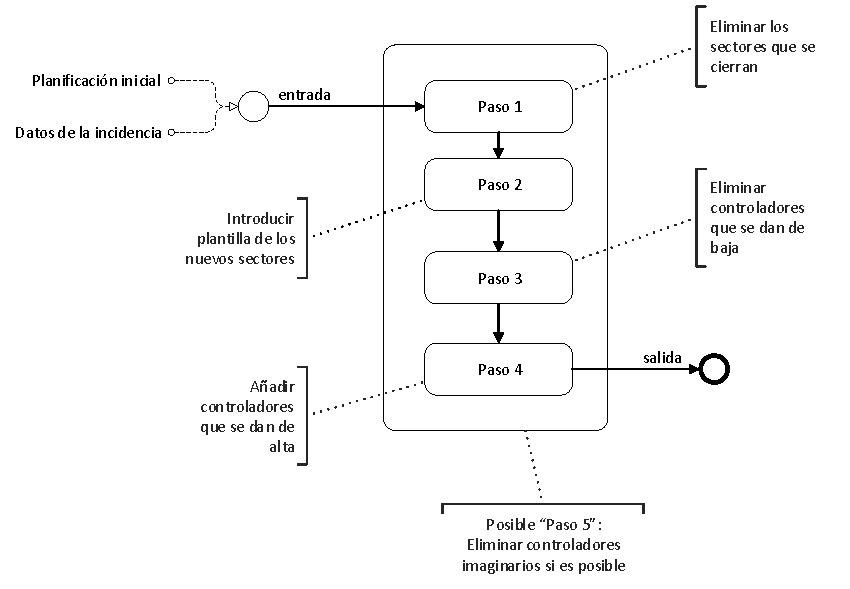
\includegraphics[width=\linewidth]{Esquema-Fase-1-extendido}
	\caption{Diagrama de flujo del funcionamiento de la Fase 1}
	\label{fig:3:esquema-fase-1}
\end{figure}

Con esos datos, la \faseuno deberá convertir la planificación inválida en una \textit{solución incial}, que emplearemos 
como punto de partida para el sistema de búsqueda inteligente que es la \fasedos{}.













